\documentclass{article}
\usepackage{amsmath}
\usepackage{physics}
\usepackage{mathtools}
\usepackage[hidelinks]{hyperref}
\usepackage[giveninits=true]{biblatex}
\usepackage{verbatim}
\usepackage{graphicx}
\usepackage{cleveref}
\usepackage{listings}
\usepackage{float}

\newfloat{lstfloat}{htbp}{lop}
\floatname{lstfloat}{Listing}
\crefname{lstfloat}{listing}{listings}

\addbibresource{{bibliography.bib}}
\def\kb#1#2{| #1 \rangle\!\langle #2 |}
\def\kbtwo#1#2#3#4{|#1 \rangle\!\langle #2 | #3 \rangle\!\langle #4 | }

\title{Implementing a quantum simulation algorithm with Qiskit}
\author{Floris van den Ende\and Sandy Bridgwater\and Antonio Mendes\and Terts Diepraam}
\date{\today}

\begin{document}

\maketitle

The aim of this project is to implement the Spectrum by Quantum Walk algorithm for the quantum chemistry problem as described by \textcite{poulin}, specifically for the hydrogen atom. The conventional method for quantum simulation is to approximate the unitary evolution operator $U = \exp{-iHt}$. This algorithm circumvents approximating $U$, thorugh the use of a different unitary operator that is also a function of the Hamiltonian. Since the new operator is function of the Hamiltonian, the energy of the system is encoded in the phase of that operator, so we can perform phase estimation to obtain the energy of the system. The new operator is defined as
i
\begin{equation} \label{W}
W = SV e^{i\pi}
\end{equation}
Where S and V are defined as
\[ S = (B (I - 2 \ket{0}\bra{0}) B^{\dagger}) \otimes I= (I-2\kb \beta \beta) \otimes I) \]
\[ V=\sum_{j}\ket{j}\bra{j} \otimes P_{j}. \]
We also define $\ket{\beta}$, which is the state we need to initialize the auxillary register in~\cite{poulin}, as
\[ \ket{\beta} = B \ket{0} = \sum_j \beta_j \ket{j}. \]
Here $\beta_j$ and $P_j$ are terms in the Hamiltonian, which, after Jordan-Wigner encoding, take the form
\begin{equation}
	\bar H = \frac H{\mathcal{N}} = \sum_j\abs{\beta_j}^2 P_j.
\end{equation}

We will simulate the hydrogen molecule, so we take the specific Hamiltonian of a hydrogen molecule which is:

\begin{align*}
\hat{H}_{B K}=&-0.81261 I+0.171201 \sigma_{0}^{z}+0.16862325 \sigma_{1}^{z}-0.2227965 \sigma_{2}^{z}+0.171201 \sigma_{1}^{z} \sigma_{0}^{z} \\
&+0.12054625 \sigma_{2}^{z} \sigma_{0}^{z}+0.17434925 \sigma_{3}^{z} \sigma_{1}^{z}+0.04532175 \sigma_{2}^{x} \sigma_{1}^{z} \sigma_{0}^{x}+0.04532175 \sigma_{2}^{y} \sigma_{1}^{z} \sigma_{0}^{y} \\
&+0.165868 \sigma_{2}^{z} \sigma_{1}^{z} \sigma_{0}^{z}+0.12054625 \sigma_{3}^{z} \sigma_{2}^{z} \sigma_{0}^{z}-0.2227965 \sigma_{3}^{z} \sigma_{2}^{z} \sigma_{1}^{z} \\
&+0.04532175 \sigma_{3}^{z} \sigma_{2}^{x} \sigma_{1}^{z} \sigma_{0}^{x}+0.04532175 \sigma_{3}^{z} \sigma_{2}^{y} \sigma_{1}^{z} \sigma_{0}^{y}+0.165868 \sigma_{3}^{z} \sigma_{2}^{z} \sigma_{1}^{z} \sigma_{0}^{z}
\end{align*}

Naively, we need a $4^4 = 256$-dimensional matrix to express this Hamiltonian. However, as there are only 16 terms, we can express this with four qubits by changing the basis to only represent 16 terms.  This means that each $\beta_j$ term corresponds to the $\ket{j}$ bitstring state.

First, we define three registers:  \verb|counting|, \verb|aux| and \verb|main|. We initialize the \verb|aux| register in the state $\ket{\beta}$. We do so by using the \verb|initialize| function of Qiskit, which takes an $n$-dimensional vector (in our case, the list of $\beta_j$ without their corresponding Pauli matrices) and initializes the $\log{n}$  qubits in the state corresponding to that vector.

Next, we have to put the \verb|main| register in the groundstate of the Hamiltonian. Usually for larger systems this is a laborious process as it requires a lot of computing power to calculate, due to the exponantially growing Hilbert space. However, hydrogen is a simple system and the groundstate can be  calculated classically via the Hartree-Fock method. We prepare this register in the groundstate by using the \verb|HartreeFock| function of the chemistry module of qiskit.

Then, we have to create the controlled-$W$ operation \cref{W} by combining the $S$ and $V$ operators. Initially, we thought that the $S$ operator had the same gate operations as the Grover Diffusion operator, found in~\cite{Qiskit-Textbook}. In that case, we could easily extrapolate the three-qubit example they gave to a four-qubit operation, by creating a four-qubit Toffoli gate with an extra ancillary qubit. Soon we realized that that is not the actual representation of $S$, as the operators are different in nature. We haven't been able to correctly implement $S$.

Similarly, we thought that the $V$ operation was just a series of tensor products of the pauli matrices from the Hamiltonian. This is also not the case, as $V$ should be a controlled operation. We don't know how to implement $V$ either.

The next step is performing phase estimation of $W$. Since we hadn't been able to implement $W$, we performed phase estimation of a random unitary. The code for phase estimation was adapted from~\cite{Qiskit-Textbook}, which is in turn based on~\textcite{nielsen}. The main complication in this part was that the original code used 3 counting qubits, instead of 2. Therefore, we adapted it to support any number of qubits. Additionally, the bits had to be adapted to fit the registry structure. After a series of controlled-$U$ operations, we apply an inverse fourier transform to the \verb|counting| register. Then the state of the counting qubits should be $\ket{\varphi}$, where $\varphi$ is the phase of $U$. Then performing measurement on the counting qubits, projected on a register of classical qubits, gives us the phase and hence the energy. A schematic of the circuit we implemented can be found in \cref{fig:full_schematic}.

\begin{figure}[htbp]
  \includegraphics[width=\linewidth]{{full_schematic.png}}
	\caption{The full circuit.}
	\label{fig:full_schematic}
\end{figure}

To run the code on a quantum computer, the circuit was significantly simplified in order to run it on 3 qubits. The result was a circuit that performs a phase estimation with a single qubit in the \verb|main| register and 2 qubits in the \verb|counting| register. After creating an account and generating an API token, we used the following code in \cref{lst:real} to run it on an IBM-Q computer. The results can be found in \cref{fig:results}. The angle that the operation in the circuit applies was smaller than our resolution, so this result was expected. All the code can be found in \url{https://github.com/FlorisvdEndeo/qiskit}.

\begin{figure}[htbp]
  \includegraphics[width=\linewidth]{{simple_schematic.png}}
	\caption{The simplified circuit.}
	\label{fig:simple_schematic}
\end{figure}

\begin{lstfloat}
\begin{lstlisting}[language=Python, frame=single]
IBMQ.load_account()
provider = IBMQ.get_provider(hub='ibm-q')
provider.backends()
backend = ibmq.least_busy(provider.backends(
    filters=lambda b: b.configuration().n_qubits >= 3
                      and not b.configuration().simulator
		      and b.status().operational==True))
job = execute(circ, backend=backend, shots=8000)
result = job.result()
\end{lstlisting}
\caption{Code for running on the IBM computer}
\label{lst:real}
\end{lstfloat}

\begin{figure}
	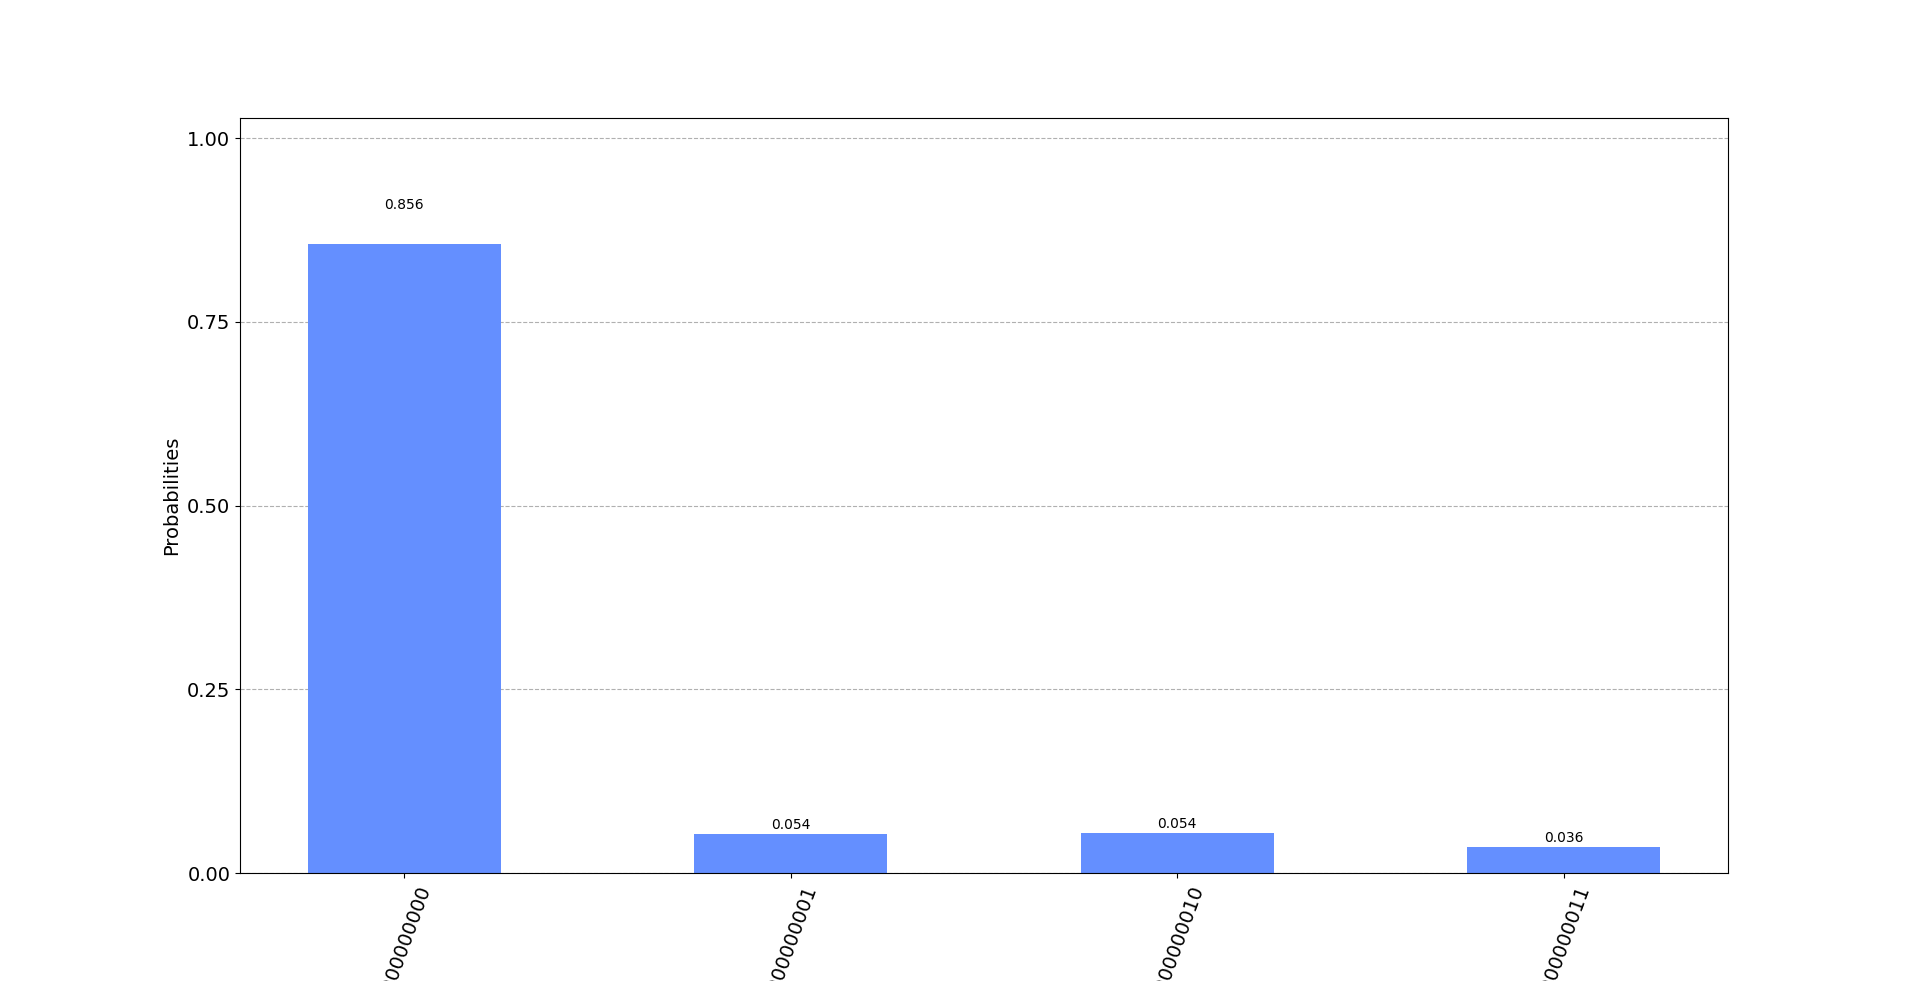
\includegraphics[width=\linewidth]{results.png}
	\caption{Results of the simplified algorithm.}
	\label{fig:results}
\end{figure}



\printbibliography
\end{document}
